\documentclass[runningheads]{llncs}
%
\usepackage{xurl}
\usepackage{graphicx}
\usepackage[portuguese]{babel}
\usepackage[utf8]{inputenc}
\usepackage{amsmath}
\usepackage{amssymb}
\usepackage{amsfonts}

\begin{document}
%
    \title{Investigação Operacional - Trabalho Prático 1}
    \author{Carlos Machado a97114, Gustavo Pereira a96867,
        Vasco Oliveira a96361, Cláudio Bessa a97063, Tiago Oliveira a97254}

    \institute{Universidade do Minho}

    \authorrunning{Carlos \and Gustavo  \and Vasco \and Cláudio \and Tiago}



    \maketitle
    \newpage
    \section{Formulação do Problema}


    Este problema ocorre quando um um veículo não tripulado tem de inspecionar linhas de transporte de energia eléctrica em alta tensão para verificar se há vegetação a interferir com as linhas. Além disso, o drone pode percorrer as arestas (linhas de alta tensão) em qualquer sentido, mas também viajar pelo ar. O objetivo principal deste desafio é fazer com que o drone percorra a menor distância possível, sendo obrigatório percorrer todas as linhas pelo menos uma vez, quer as linhas que pertencem originalmente do mapa, quer as linhas que devemos adicionar de modo a formar um caminho euleriano.

    O maior número de estudante do grupo é 97254, o que significa que teremos de retirar as arestas C e E do mapa inicial.

    \begin{figure}[h]
        \centering
        \includegraphics[scale=0.45]{drone.png}
        \caption{Mapa de linhas de alta tensão.}
        \label{fig:data1}
    \end{figure}

    O percurso que o drone tem de percorrer denomina-se de caminho Euleriano. Este caminho apenas existe quando os vértices interiores ao mapa tem grau de entrada/saída par, e os vértices que representam o início (I) e o final (F) do percurso grau ímpar. Na Figura 2, encontram-se assinalados os vértices onde é necessário aumentar o grau, ou seja, a criação de novas arestas. Desta forma, surge um problema de programação linear onde devemos adicionar arestas tentando otimizar o itenerário de modo a minimizar a distãncia percorrida.



    \newpage

    \section{Modelo}

    \begin{figure}[h]
        \centering
        \includegraphics[scale=0.25]{arestasgrau.jpg}
        \caption{Vértices com grau insuficiente.}
        \label{fig:data2}
    \end{figure}

    \subsection{Variáveis de decisão}

    $xij$: existe ou não uma aresta a unir os vértices $i,j \in \{I,1,2,3,4,6,7,9,10,11,12,F\}$, onde $xij \in \{0,1\}$.

    \newpage

    \subsection{Parâmetros}

    $dij$ : comprimento da aresta que une os vértices i e j.
    Os comprimentos de todas as arestas podem ser calculados a partir da seguinte tabela:

    \begin{figure}[h]
        \centering
        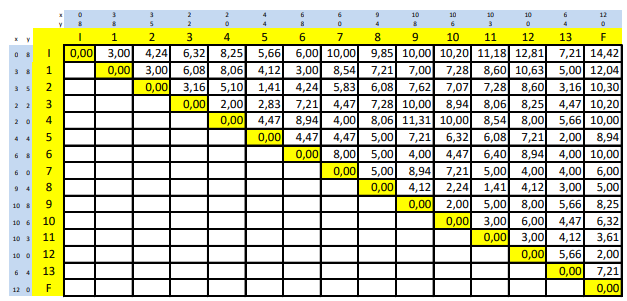
\includegraphics[scale=0.75]{distancias euclidianas.PNG}
        \caption{Distancias Euclidianas fornecidas}
        \label{fig:data3}
    \end{figure}

    \subsection{Função objetivo}
    Minimização da distância percorrida pelo \textit{drone}.
    \newline \textit{min} : $\sum_{i,j}^{} \in V,  dij  \times    xij,  i < j$


    \newpage
    \subsection{Restrições}
    Cada vértice apenas deve fazer parte de uma só aresta.
    \newline $\forall i \in V \wedge  j \in V,  \sum xij = 1, i < j$

    \begin{figure}[ht]
        \centering
        \includegraphics[scale=0.4]{lpsolve code.PNG}
        \caption{Ficheiro de input LPSolve}
        \label{fig:data4}
    \end{figure}

    \newpage

    \section{Solução ótima}
    Introduzimos os modelo criado no LPSolve e descobrimos as arestas a adicionar no
    percurso: $I-1; 2-6; 3-4; 7-11; 9-10; 12-F$. No final o percurso ficou com um comprimento total de 18.24\textit{(u.c)}.

    \begin{figure}[ht]
        \centering
        \includegraphics[scale=0.8]{lpsolve result zoom.png}
        \caption{Output retornado pelo LPSolve}
        \label{fig:data5}
    \end{figure}

    \begin{figure}[ht]
        \centering
        \includegraphics[scale=0.2]{arestasadicionais.jpg}
        \caption{Arestas contempladas como solução ótima}
        \label{fig:data6}
    \end{figure}

    \newpage


    \clearpage

    \textbf{Exemplo de percurso}:
    \newline $I-4-3-2-1-I-1-6-2-5-3-4-7-13-6-9-10-8-11-7-12-F-12-11-10-9-F$

    \begin{figure}[h]
        \centering
        \includegraphics[scale=0.25]{caminho.jpg}
        \caption{Percurso Possível}
        \label{fig:data7}
    \end{figure}

    \section{Validação do modelo}

    provar que é solução ótima, com um modelo alternativo?




\end{document}
